\documentclass[]{article}
\usepackage[margin=4cm]{geometry}
\usepackage[utf8]{inputenc}
\usepackage{graphicx}
\usepackage{amsfonts}
 
\title{Robust Reinforcement Learning}
\author{Mathias Beguin}
\date{2018}
 
\begin{document}
 
\begin{titlepage}
\maketitle
\end{titlepage}

\section{Formalization of the problem}
Reinforcement learning (abbreviated RL) is an area of machine learning in which agents learn how to interact in an environment so as to maximize a notion of reward. It differs from standard supervised learning in that correct input/output pairs need not be presented, and sub-optimal actions need not to be explicitly corrected. Instead it focuses on performance which involve finding a balance between exploration of uncharted state and exploitation of current knowledge.


\subsection{Markov Decision Process} \label{section:MDP}
In reinforcement learning, the problem is usually described as a Markov Decision Process. It is a mathematical framework used to model decision making problem in which outcomes are under the control of an agent. It is defined as a 5-tuple $(S, A, P_a, R_a, \gamma)$ where
\begin{itemize}
	\item $S$ is a set of states
	\item $A$ is a set of actions ($A_s$ is the set of available actions in state $s$)
	\item $Pr(s_{t+1} = s' | s_t = s, a_t = a)$ is the probability of transition from state $s$ to state $s'$ under the action $a$ at time $t$
	\item $R(s, a, s')$ is the immediate reward after a transition from $s$ to $s'$ by taking the action $a$
	\item $\gamma \in [0, 1)$ is the discount factor, which represents the difference in importance between future and present rewards
\end{itemize}

A reinforcement learning agent interacts with its environment in discrete time steps. At each time $t$, the agent receives an observation $o_{t}$. It then chooses an action $a_{t}$ from the set of available actions, which is subsequently sent to the environment. The environment moves to a new state $s_{t+1}$ and the reward $r_{t}$ associated with the transition $(s_{t},a_{t},s_{t+1})$ is determined.

\begin{figure}[h]
	\centering
	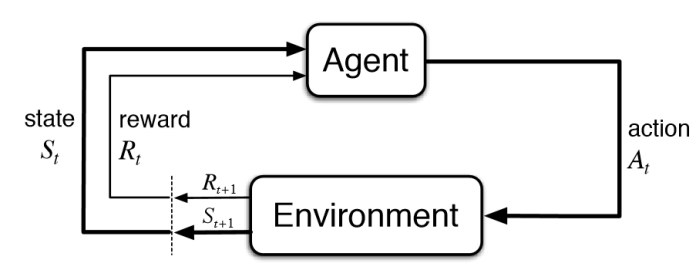
\includegraphics[scale=0.5]{rl-loop.jpg}
	\caption{Reinforcement learning interaction loop}
\end{figure}


The goal of a reinforcement learning agent is to learn a policy $\pi$ that specifies the action $\pi(s)$ to take in state $s$. This policy should maximize some cumulative function of the rewards. Typically the expected discounted sum of rewards $\sum_{t = 0}^{\infty} \gamma^t R(s, a_t, s')$ where $a_t = \pi(s)$ is taken.

\subsection{Policy Gradient}
Policy based models are methods that learn a parameterized policy $\pi (a | s; \theta)$ that can select actions without consulting a value function. A value function may still be used to learn the policy parameter, but is not required for action selection. They work by computing an estimator

\begin{equation}
\hat{g} = \hat{\mathbb{E}}_t [\nabla_\theta \ log\ \pi_\theta(a_t | s_t) \hat{A}_t]
\end{equation}

 using trajectories generated by the policy and plugging it into a stochastic gradient ascent algorithm. The term $\hat{A}_t$ corresponds to an estimator of the advantage function at time step $t$. It has for purpose to determine which action yields better or worse result than the average. When an estimator of the value function $V_\pi(s) = E[\sum_{t = 0}^{\infty} \gamma^tr_t | s_0 = s]$ is used, the methods become \textit{actor-critic methods}.

\subsection{Contribution}
The goal of this thesis is to augment the initial goal of learning a parametrized policy so as to make it robust to the value of nuisance parameters $z \in Z$. 
Inspired by the work of Gilles Louppe, Michael Kagan and Kyle Cranmer in "Learning to Pivot with Adversarial Networks", our data generation process is a Markov Decision Process defined as in section \ref{section:MDP} where we modify the transition probability distribution to introduce the nuisance parameters and it becomes $Pr(s_{t+1} | s_t, a_t, z)$.

To learn such policy, we need it to be a pivot with respect to $Z$. A pivot is  a quantity whose distribution is invariant with the nuisance parameters. Therefore, we would like to learn policies such that

\begin{equation}
\pi (a | s, z; \theta) = \pi (a | s, z'; \theta)
\end{equation}

for all $z$, $z' \in Z$, all values of $a \in A$ and all values of $s \in S$. This equation implies that $\pi(a | s, \theta)$ and $Z$ are independent random variables.

\subsection{Method}
Following the method of "Learning to Pivot", we use a re-purposed adversarial networks as a means to constrain the policy $\pi$. We pit $\pi$ against an adversarial model $r$ that takes as input a sequence of tuples $\tau = (s_t, a_t, r_t, s_{t+1})$ where $t \in [0, T]$ which correspond to an episode and where the $a_t$ are chosen using $\pi(a | s;\theta)$ and  outputs a function modeling the posterior probability $z$ given $\tau$:

\begin{equation}
r := Pr(z | \tau \sim \pi(a | s;\theta))
\end{equation}


Intuitively, if $\pi (a | s, z; \theta)$ varies with $z$, then the corresponding correlation can be captured by $r$. By contrast, if $\pi (a | s, z; \theta)$ is invariant with $z$, then $r$ should perform poorly and be close to random guessing.


 
\end{document}